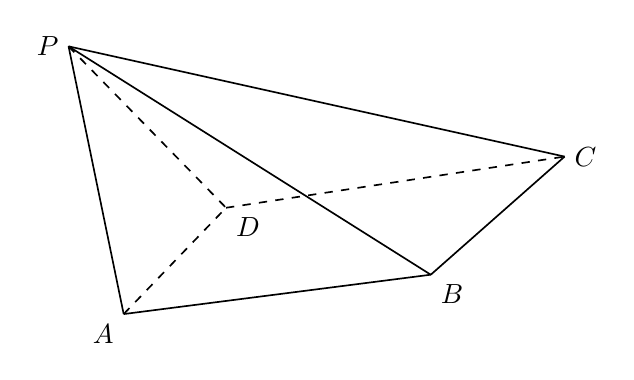
\begin{tikzpicture}[line width=.6pt]
  \coordinate (P) at (0,3.4);
  \coordinate (A) at (0.7,0);
  \coordinate (B) at (4.6,0.5);
  \coordinate (C) at (6.3,2.0);
  \coordinate (D) at (2.0,1.35);
  \draw[dashed] (P) -- (D);
  \draw[dashed] (A) -- (D);
  \draw[dashed] (D) -- (C);
  \draw (P) -- (A);
  \draw (P) -- (C);
  \draw (P) -- (B);
  \draw (A) -- (B);
  \draw (B) -- (C);
  \node[left] at (P) {$P$};
  \node[below left] at (A) {$A$};
  \node[below right] at (B) {$B$};
  \node[right] at (C) {$C$};
  \node[below right] at (D) {$D$};
\end{tikzpicture}
